\chapter{調和振動子の量子力学}

前章の議論では、ショット雑音や増幅器雑音を現象論として与えた。これらの式を用いれば、それを元に光信号の信号対雑音比の評価を行うことができる。一方、なぜ、どういう場合にこれらの式が成り立つのか、という問いに答えるには、その背後にある物理を考える必要がある。それが量子光学である。
	
量子光学では、光の場を多数の空間モードおよび時間/周波数モードに分解し、ひとつひとつのモードを量子力学的な調和振動子とみなす。複数のモードの量子状態を規定し、それに対してある物理量の測定を行うことで、物理量の期待値およびその揺らぎを求める。このような枠組みのもとで、光子の集まりとしての光の振る舞いを記述することができる。

本章では、調和振動子の量子力学の基本についておさらいをしておこう。


\section{調和振動子}
ばねと重りからなる、減衰のない調和振動子を考え、そのばね定数を$k$、重りの質量を$m$としよう。振動子の共振角周波数は$\omega = \sqrt{k/m}$である。また、重りの位置の平衡点からのずれを$q$と表す。ここで、ばねのエネルギーを
\begin{equation}
	\frac{k}{2}x^2 \equiv \frac{1}{2}(\omega q)^2
\end{equation}
と表し、振動子の運動エネルギーを
\begin{equation}
	\frac{m}{2}\left(\frac{dx}{dt}\right)^2\equiv\frac{1}{2}p^2
\end{equation}
と表そう\footnote{本来ならばばねのエネルギーは$\frac 1 2 m\omega_0^2 x^2$、運動エネルギーは$p^2/2m$とするべきだが、この後で調和振動子を光の場に対応させる際に、光には重さがないのでつじつまが合わないため、$m = 1$とし、光には$\hbar k$の運動量があることを前提条件として話を進める。}。
図\ref{fig:classical_phase_space}(a)に示すように、$q$を横軸に、$p$を縦軸として振動子の状態を表す。このような2次元平面を位相平面という。振動子の運動エネルギーとポテンシャルエネルギーの和は一定であることから、時間発展とともに右回りの円の軌跡を描く。

あとで示すように、量子力学では位置や運動量が広がりを持つ確率分布として与えられる。イメージとしては図\ref{fig:classical_phase_space}(b)のようになる。ただし、この図はあくまでイメージであって、そのまま信じてはいけない。揺らぎの様子は、位置だけを測定するのか、位置と運動量を同時に測定するのかによって変わって来る。また、量子力学では、位相が確定しない状態等、様々な状態が存在しうる。

\begin{figure}
  \centering
  \includegraphics[width=9cm]{fig/2-1_phase_space.eps} 
  \caption{位相平面における調和振動子の位置と運動量の時間発展。(a) 古典的な調和振動子。(b) 量子的な調和振動子。}
  \label{fig:classical_phase_space}
\end{figure}


\section{シュレディンガー方程式とハイゼンベルグの運動方程式}
量子力学では、系の量子状態を状態ベクトル\footnote{波動関数、量子状態とも同じ。}で表すとともに、位置$q$や運動量$p$をエルミート演算子$\hat q, \hat p$で表すことでシュレディンガー方程式を立て、それを解いていく。詳細は付録を参照してほしい。なぜ演算子で表すのかというと、位置や運動量に揺らぎ、もしくは不確定性があるからである。調和振動子がある量子状態にあったとすると、位置も運動量も確率分布としてしか知ることはできない。このとき、量子状態から確率分布を抽出する操作を、演算子で表現する。また、演算子は位置や運動量のような物理量を表す際だけでなく、量子状態に変化を与える際にも用いる。

本節では、シュレディンガー方程式が状態ベクトルの時間変化を記述する方程式であることを説明する。このように状態ベクトルを時間発展させていく描像を「シュレディンガー描像」という。また、時間発展操作を加える演算子である時間発展演算子を導入する。
さらに、状態ベクトルを時間発展させるのではなく、演算子を時間発展させる計算方法である「ハイゼンベルグ描像」について説明するとともに、演算子の時間発展を表す方程式であるハイゼンベルグの運動方程式を導入する。

後の章で説明するように、時間発展演算子やハイゼンベルグの運動方程式は、時間発展以外の操作にも使うことができる。これによって、光の発生、検出、増幅等の計算が極めてシンプルになる。一方で、これらの計算を理解する上で、シュレディンガー描像のことを表しているのか、ハイゼンベルグ描像のことを表しているのかをきちんと押さえておくことが重要である。

\subsection{シュレディンガー方程式と時間発展演算子}
時間とともに変化する状態ベクトル$\ket{\Psi(t)}$の時間変化を記述する方程式
\begin{equation}
  i\hbar \frac{d}{dt}\ket{\Psi(t)} = \hat H \ket{\Psi(t)}
  \label{eq:Schrodinger_equation}
\end{equation}
を\textbf{シュレディンガー方程式}という。この式の左辺は、状態ベクトルの時間微分を$i\hbar$倍したものである。右辺は、エネルギーを表す演算子(ハミルトニアン)を状態ベクトルに作用させたものである。

$\hat H$が時間変化しない場合、式(\ref{eq:Schrodinger_equation})は簡単に解くことができる。まず、微分を微小時間$\Delta t$での差分に置き換えると、
\begin{equation}
  	\ket{\Psi(\Delta t)} - \ket{\Psi(0)} \sim \frac{\Delta t}{i\hbar}\hat H \ket{\Psi(0)}
\end{equation}
より、
\begin{equation}
  \ket{\Psi(\Delta t)} \sim \left( 1 + \frac{\hat H}{i\hbar}\Delta t\right)\ket{\Psi(0)}
\end{equation}
であるから、次式を得る。
\begin{equation}
  \ket{\Psi(N\Delta t)}\sim \left(1 + \frac{\hat H}{i\hbar}\Delta t\right)^N\ket{\Psi(0)}
\end{equation}
ここで、$t = N\Delta t$として$N \to \infty$の極限を取ると、シュレディンガー方程式の解として次式が得られる。
\begin{equation}
  \ket{\Psi(t)} = \exp \left( \frac{\hat H}{i\hbar}t \right) \ket{\Psi(0)}
  \label{eq:Schrodinger_solution}
\end{equation}
である。ここで、$\hat H$の固有ベクトルを$\ket{\Psi_k}$、エネルギー固有値を$E_k$とすれば、$\hat H \ket{\Psi_k (0)}=E_k\ket{\Psi_k (0)}$であるから、これを(\ref{eq:Schrodinger_solution})に代入すると
\begin{equation}
  \ket{\Psi_k(t)} = \exp\left(-i\frac{E_k}\hbar t\right)\ket{\Psi_k(0)}
  \label{eq:time_evolution_of_steady_state}
\end{equation}
を得る。すなわち、式(\ref{eq:Schrodinger_solution})は、各エネルギー固有状態を、各エネルギーに対応する周波数$\omega_k = E_k / \hbar$で時間とともに位相回転させている。これはドブロイの関係式$E = \hbar \omega$を表したものである、と考えることもできる。

ここで、式(\ref{eq:Schrodinger_solution})に現れる
\begin{equation}
  \hat U(t) \equiv \exp \left( \frac{\hat H}{i\hbar} t \right)
\end{equation}
を\textbf{時間発展演算子}といい、$\ket{\Psi(t)} = \hat U(t) \ket{\Psi(0)}$である。また、$\hat U ^\dagger (t) = \hat U(-t)$であるから、$\hat U^\dagger \hat U = \pmb 1$となり、時間発展演算子がユニタリであることがわかる
\footnote{時間発展演算子がユニタリであることは、波動関数のノルムを変化させない、すなわち、粒子の存在確率を変化させないことに対応している
。これは、エルミート演算子であるハミルトニアンの固有値(エネルギー固有値)が実数であるために、式(\ref{eq:time_evolution_of_steady_state})において各固有ベクトルの振幅が時間とともに変化しないこととも対応している。}。
%\footnote{$\hat H$が時間とともに変化する場合も、時間発展演算子を求めることができ、やはりユニタリ行列となる。}

\subsection{シュレディンガー描像とハイゼンベルグ描像}
振動子の変位のように、時間とともに変化する物理量の期待値を計算することを考えよう。この時、状態ベクトルが時間とともに変化するとして考えると、その期待値$\braket{\hat A}$は
\begin{equation}
  \braket{\hat A} = \braket{\Psi(t)|\hat A | \Psi(t)}
  \label{eq:Schrodinger_picture}
\end{equation}
として計算することができる\footnote{付録のA.2節を参照のこと。}。

一方、状態ベクトルに対し、時間発展演算子を作用させることで時間発展を表すと、
\begin{equation}
  \braket{\Psi(t)|\hat A|\Psi(t)} = \braket{\Psi(0)|\hat U^\dagger(t) \hat A \hat U(t) | \Psi(0)} \equiv \braket{\Psi(0) | \hat A_\mathrm H(t) | \Psi(0)}
  	\label{eq:Heisenberg_picture}
\end{equation}
と表すことができる。

式(\ref{eq:Schrodinger_picture})のように、時間とともに状態ベクトルを変化させて時間変化を考えることを、\textbf{シュレディンガー描像}\index{しゅれでぃんがーびょうぞう@シュレディンガー描像}という。一方、式(\ref{eq:Heisenberg_picture})のように物理量の演算子を変化させることで時間変化を考えることを\textbf{ハイゼンベルグ描像}\index{はいぜんべるぐびょうぞう@ハイゼンベルグ描像}という。

シュレディンガー描像は、波動関数の時間発展を直感的に捉える上で有用である。一方、光の量子論では、ハイゼンベルグ描像を用いて、演算子を変化させて様々な状況を計算することが多用される。

ハイゼンベルグ描像では、時間発展を以下のようにして計算する。
\begin{equation}
\begin{aligned}
  \frac{d}{dt}\hat A_\mathrm H (t) &= \left( \frac d {dt} \hat U^\dagger (t)\right) \hat A \hat U(t) + \hat U^\dagger \hat A \left( \frac{d}{dt}\hat U(t) \right)\\
	&= \frac{-\hat H}{i\hbar} \hat U^\dagger (t)\hat A\hat U(t) + \frac{1}{i\hbar}\hat U^\dagger(t) \hat A \hat U(t) \hat H\\
	&= \frac{i}{\hbar}\left( \hat H \hat A_\mathrm H(t) - \hat A_\mathrm H(t) \hat H \right) = \frac{i}{\hbar}\left[ \hat H, \hat A_\mathrm H \right]
\label{eq:Heisenberg_equation_of_motion}
\end{aligned}
\end{equation}
ただし、$\hat H$が時間と共に変化しないことを仮定した。また、$\hat H$と$\hat U$が交換可能であることを用いた\footnote{$\hat U$をテーラー展開すれば、$\hat H$の多項式で表せる。このことから$\hat U$と$\hat H$が交換可能であることがわかる。}。この式(\ref{eq:Heisenberg_equation_of_motion})を\textbf{ハイゼンベルグの運動方程式}\index{はいぜんべるぐのうんどうほうていしき@ハイゼンベルグの運動方程式}という。

\section{調和振動子のシュレディンガー方程式とその解}
ここまでで述べてきたように、古典的な調和振動子は、位置$q$と運動量$p$の平面(位相平面)における回転運動として表される。また、量子論では、位置と運動量を演算子$\hat q$と$\hat p$で表す。調和振動子では、計算をシンプルにするために、消滅・生成演算子$\hat a, \hat a^\dagger$を導入する。本節では、消滅・生成演算子を用いて、調和振動子の解を求める。光の量子論では、この生成・消滅演算子が重要な役割を果たす。

\subsection{調和振動子のハミルトニアンと生成・消滅演算子}
調和振動子のエネルギーは、位置エネルギー$\frac{1}{2}(\omega \hat q)^2 $と運動エネルギー$\frac{1}{2}\hat p^2 $の和である。エネルギー演算子であるハミルトニアンは、
\begin{equation}
  \hat H = \frac{1}{2}(\omega \hat q)^2 + \frac 1 2 \hat p^2
\end{equation}
と表される。ここで、式を簡略化するために、規格化した位置および振幅の演算子$\hat P, \hat Q$を用いて、
\begin{equation}
  \hat H = \frac 1 2 \hbar \omega (\hat Q ^2 + \hat P^2)
\end{equation}
と表そう。このような置き換えは、
$\hat Q = \sqrt \frac{\omega}{\hbar} \hat q$, 
$\hat P = \frac{1}{\sqrt{\hbar \omega}}\hat p$と
おくことによって可能である。また、この$\hat Q$, $\hat P$に対しては以下の交換関係が成り立つ。
\begin{equation}
  [\hat Q, \hat P] = \left[\sqrt{\frac{\omega}{\hbar}}\hat q, \frac{1}{\sqrt{\hbar \omega}}\hat p \right] = \frac{1}{\hbar}[\hat q, \hat p] = i
  \label{eq:commutation_Q_P}
\end{equation}
ただし、$[\hat q, \hat p] = i\hbar$は量子論の要請である\footnote{詳細は\ref{section:commutation}節を参照されたい。}。

ここでさらに、複素振幅の演算子である$\hat a$を次式で定義する。
\begin{equation}
  \hat a = \frac{1}{\sqrt 2}(\hat Q + i\hat P)
  \label{eq:annihilation_operator}
\end{equation}
このとき、$\hat a$のエルミート共役は次式で与えられる。
\begin{equation}
  \hat a^\dagger = \frac{1}{\sqrt 2}(\hat Q - i\hat P)
  \label{eq:creation_operator}
\end{equation}
ただし、ここでは$\hat Q$および$\hat P$がエルミートであること、すなわち$\hat Q^\dagger = \hat Q$, $\hat P^\dagger = \hat P$であることを用いた。

$\hat a$は\textbf{消滅演算子}、$\hat a^\dagger$は\textbf{生成演算子}と呼ばれ、以下のような様々な性質を持つ。
\subsubsection{非エルミート性}
明らかに$\hat a^\dagger \neq \hat a$であるから、$\hat a^\dagger$、$\hat a$はエルミート演算子ではない。このため、$\hat a$は量子力学において誤差なく測定可能な物理量ではない。一方、後で議論するように一定の誤差を許せば、$\hat a$が表す物理量(複素振幅)を測定することは可能である。

\subsubsection{交換関係}
生成・消滅演算子は交換せず、次式が成り立つ。
\begin{equation}
  [\hat a, \hat a^\dagger] = \hat a \hat a^\dagger - \hat a^\dagger \hat a = 1
\end{equation}
証明は以下の通り。
式(\ref{eq:creation_operator}), (\ref{eq:annihilation_operator}), (\ref{eq:commutation_Q_P})を用いて次式を得る。
\begin{equation}
\begin{aligned}
  \left[\hat a , \hat a^\dagger\right] &= \frac{1}{2}\left\{(\hat Q + i\hat P)(\hat Q - i\hat P) - (\hat Q - i\hat P)(\hat Q + i\hat P)\right\} \\
  &= i(\hat P\hat Q - \hat Q\hat P) = -i[\hat Q, \hat P] = 1
\end{aligned}
\end{equation}

\subsubsection{生成・消滅演算子によるハミルトニアンの表現}
$\hat Q$, $\hat P$で表される演算子は全て生成・消滅演算子で表すことができる。実際、調和振動子のハミルトニアンは次式のように書ける。
\begin{equation}
  \hat H = \frac{\hbar \omega}{2}(\hat Q^2 + \hat P^2) = \frac{\hbar \omega}{2}(\hat a^\dagger \hat a + \hat a \hat a^\dagger) = \hbar \omega\left(\hat a^\dagger \hat a + \frac 1 2\right)
\end{equation}
ただし、$\hat Q = (\hat a + \hat a^\dagger)/\sqrt 2$, $\hat P = (\hat a - \hat a^\dagger) / i\sqrt 2$を用いた。

また、$\hat H$と$\hat a$, $\hat a^\dagger$は以下のような交換関係を有する。
\begin{equation}
\begin{aligned}
  \left[\hat H, \hat a\right] &= [\hbar \omega (\hat a^\dagger \hat a + 1/2), \hat a] = \hbar \omega [\hat a^\dagger \hat a, \hat a] = \hbar \omega (\hat a^\dagger \hat a \hat a - \hat a \hat a^\dagger \hat a)\\ 
  &= \hbar \omega (\hat a^\dagger \hat a \hat a - (\hat a^\dagger \hat a + 1) \hat a) = -\hbar\omega \hat a
\end{aligned}
\end{equation}
\begin{equation}
  \begin{aligned}
  	\left[\hat H, \hat a^\dagger \right] &= [\hbar \omega (\hat a^\dagger \hat a + 1/2), \hat a^\dagger] = \hbar \omega [\hat a^\dagger \hat a, \hat a^\dagger] = \hbar \omega (\hat a^\dagger \hat a \hat a^\dagger - \hat a^\dagger \hat a^\dagger \hat a)\\ 
  &= \hbar \omega (\hat a^\dagger (\hat a^\dagger \hat a + 1) - \hat a^\dagger \hat a^\dagger\hat a) = \hbar\omega \hat a^\dagger
  \end{aligned}
\end{equation}
これらの交換関係は、ハイゼンベルグ描像における時間発展の計算に用いられる。

\subsection{消滅演算子の実部および虚部の演算子}
$\hat a$の実部および虚部の演算子を次式で定義する。
\begin{equation}
  \begin{aligned}
  	\hat a_1 &\equiv \frac 1 2 (\hat a + \hat a^\dagger) = \frac 1 {\sqrt 2} \hat Q\\
  	\hat a_2 &\equiv \frac 1 {2i} (\hat a - \hat a^\dagger) = \frac 1 {\sqrt 2} \hat P
  \end{aligned}
\end{equation}
これらはいずれもエルミートである\footnote{$\hat a_1^\dagger = \hat a_1, \hat a_2^\dagger = \hat a_2$であることは定義からすぐわかる。}。このことから、$\hat a_1$および$\hat a_2$は固有状態と固有ベクトルを有し、物理量の計測が可能である。

ただし、$\hat a_1$と$\hat a_2$を同時に測定することはできない。これは、
\begin{equation}
  \left[ \hat a_1, \hat a_2\right] = \frac 1 2 [\hat Q, \hat P] = \frac i 2
\end{equation}
であることによる。


\subsection{生成・消滅演算子の時間発展}
前節で述べたように、ハイゼンベルグ描像では演算子が時間発展する。ハイゼンベルグの運動方程式より、
\begin{equation}
  \frac{d}{dt}\hat a(t) = \frac{i}{\hbar}[\hat H, \hat a(t)] = -i\omega \hat a(t)
\end{equation}
であるから、次式を得る。
\begin{equation}
  \hat a(t) = e^{-i\omega t}\hat a(0)
\end{equation}
同様に、$\hat a^\dagger$に対しては次式が成り立つ。
\begin{equation}
  \hat a^\dagger(t) = e^{i\omega t}\hat a^\dagger(0)
\end{equation}
これらの式からも、$\hat a$が複素振幅に対応する演算子であることが見て取れる。

\subsection{調和振動子の解}
以上の準備を踏まえて、調和振動子の解となる状態ベクトルは以下のように表すことができる。

$\hat H$のエネルギー固有状態は、非負の整数$n = 0, 1, 2, \hdots$を用いて$\ket n$と表すことができ、そのエネルギー固有値は
\begin{equation}
  E_n = \hbar \omega \left(n + \frac 1 2\right)
  \label{eq:energy_of_eigenstate}
\end{equation}
で与えられる。この$\ket n$の線形結合で表される
\begin{equation}
  \ket \phi = \sum_{k = 0}^{\infty} c_k\ket k
  \label{eq:superposition_of_eigenstate}
\end{equation}
が調和振動子の解となる。ただし、$\ket n$は規格化されている。また、$\sum_{k = 0}^\infty |c_k|^2 = 1$である。

このことは以下のような手続きで示すことができる。まず、「$\ket n$は$\hat a^\dagger \hat a$の固有ベクトルで、その固有値が$n$となる」ことを仮定すると、$n$が非負となることを示そう。この仮定は、
\begin{equation}
  \hat a^\dagger \hat a \ket n = n\ket n
\end{equation}
と表せる。ここで、左から$\bra n$をかけると、
\begin{equation}
  \bra n \hat a^\dagger \hat a \ket n = n \braket {n|n} = n
\end{equation}
ここで、$(\hat a \ket n)^\dagger = \bra n \hat a^\dagger$であることから、$\bra n \hat a ^\dagger \hat a \ket n = \| \hat a \ket n \|^2 \geq 0$を満たす。したがって、$n \geq 0$である。

また、$n$が整数であることは以下のように示すことができる。まず、$\ket n$に$\hat a$を作用させたものが$\hat a^\dagger\hat a$の固有ベクトルであることが以下のようにわかる。
\begin{equation}
	\begin{aligned}
		\hat a^\dagger \hat a \hat a \ket n &= (\hat a \hat a^\dagger -1)\hat a \ket n\\
		&= (\hat a \hat a^\dagger \hat a - \hat a)\ket n\\
		&= (n - 1)\hat a\ket n
	\end{aligned}
\end{equation}
このように、$\hat a \ket n$に対応する固有値が$n - 1$であることから、$\hat a \ket n \propto \ket {n - 1}$である。その比例定数を$L_n$として、
\begin{equation}
  \hat a \ket n = L_n\ket{n-1}
\end{equation}
としよう。このエルミート共役は
\begin{equation}
  \bra n \hat a^\dagger = L_n^*\bra{n-1}
\end{equation}
であるから、この2式を掛け合わせて次式を得る。
\begin{equation}
  |L_n|^2\braket{n-1|n-1} = \bra n \hat a^\dagger \hat a \ket n = n \braket{n|n}
\end{equation}
$\ket n$は規格化されているから、$|L_n|^2 = n$より$L_n = \sqrt n e^{i\theta}$ ($\theta$は実数)を得る。このように$L_n$には複素数の偏角だけの不確定性があるが、これは$\hat a$の時間発展に伴って偏角が変化することと対応しているので、$\theta = 0$として良い。最終的に次式を得る。
\begin{equation}
  \hat a \ket n = \sqrt n \ket {n - 1}
  \label{eq:annihilation_operator_normalization}
\end{equation}

同様に、$\ket n$に$\hat a ^\dagger$を作用させたものも$\hat a^\dagger \hat a$の固有ベクトルであることを示すことができる。
\begin{equation}
	\begin{aligned}
		\hat a^\dagger \hat a \hat a^\dagger \ket n &= \hat a ^\dagger (\hat a^\dagger \hat a + 1) \ket n\\
		&= (n + 1)\hat a^\dagger\ket n
	\end{aligned}
\end{equation}
したがって、$\hat a^\dagger \ket n$の固有値は$n + 1$である。このことから、$\hat a^\dagger \ket n \propto \ket {n + 1}$である。その比例定数を$K_n$として、
\begin{equation}
  \hat a^\dagger \ket n = K_n\ket{n+1}
\end{equation}
としよう。このエルミート共役は
\begin{equation}
  \bra n \hat a = K_n^*\bra{n+1}
\end{equation}
であるから、この2式を掛け合わせて次式を得る。
\begin{equation}
  |K_n|^2\braket{n+1|n+1} = \bra n \hat a\hat a^\dagger \ket n = \bra n (\hat a^\dagger \hat a + 1) \ket n = (n + 1) \braket{n|n}
\end{equation}
$\ket n$は規格化されているから、$|K_n|^2 = n + 1$より、$K_n = \sqrt {n+1} e^{i\theta}$ ($\theta$は実数)を得る。$L_n$と同様に$K_n$にも複素数の偏角だけの不確定性があるが、これは$\hat a^\dagger$の時間発展に伴って偏角が変化することと対応しているので、$\theta = 0$とおいて良い。最終的に次式を得る。
\begin{equation}
  \hat a^\dagger \ket n = \sqrt {n + 1} \ket {n + 1}
    \label{eq:creation_operator_normalization}
\end{equation}

式(\ref{eq:creation_operator_normalization}), (\ref{eq:annihilation_operator_normalization})から、$\hat a^\dagger$、$\hat a$ はそれぞれ$n$の番号を1だけ上げる、もしくは下げる演算子であることがわかる。これが、$\hat a^\dagger$を生成演算子、$\hat a$を消滅演算子と呼ぶ理由である。

ここで、式(\ref{eq:annihilation_operator})において$n = 0$とおくと、$\hat a\ket 0 = 0 \ket {-1}$となり、$\ket 0$よりも小さな$n$に対して$\ket n$を作ることができない。このことは$n$が非負である、という条件を満たしている。

また、整数以外の$n$に対して$\ket n$が存在すると仮定すると、$\hat a$を作用させていった時に、$n < 0$に対しても$\ket n$が存在することになり、$n$が非負である、という条件を満たさない。このことから、$n$は整数でなければならないことがわかる。

逆に、$\ket 0$に$\hat a^\dagger$を作用させると、任意の整数$n$に対して$\ket n$を作ることができる。すなわち
\begin{equation}
  \ket n = \frac 1 {\sqrt n} \hat a^\dagger \ket {n - 1} 
  = \frac 1 {\sqrt{n(n-1)}} (\hat a^\dagger)^2\ket{n - 2} = \cdots 
  = \frac{1}{\sqrt{n!}}(\hat a^\dagger)^n\ket 0
\end{equation}
である。以上のことから、$\hat a^\dagger a$の固有状態は$\ket n$でその固有値は$n$であることを示すことができる。

同様にハミルトニアンの固有状態も$\ket n$であり、その固有値が式(\ref{eq:energy_of_eigenstate})で与えられることもただちにわかる。
\begin{equation}
  \hat H \ket n = \hbar \omega (\hat a^\dagger \hat a + 1/2)\ket n = \hbar \omega (n + 1/2)\ket n
\end{equation}

次の章で述べるように、量子光学では、あるモードに$n$個の光子が存在する状態を、調和振動子の$\ket n$に対応させる。

\begin{comment}
\begin{equation}
\begin{aligned}
  \hat H \hat a\ket n &= (\hat a \hat H - \hbar \omega \hat a)\ket n \\
  &= \left\{ \hat a \hbar \omega (\hat a^\dagger \hat a + 1/2) - \hbar \omega \hat a\right\}\ket n\\ 
  &= \left\{ \hat a \hbar \omega (n - 1 + 1/2) - \hbar \omega \hat a\right\}\ket n\\ 
\end{aligned}
\end{equation}
\end{comment}

\subsection{調和振動子のエネルギー固有状態}
$\ket n$が調和振動子のエネルギー固有状態であることは上で述べた。これだけだとイメージが湧きにくいので、$Q$表示における具体的な形を示しておこう。

$Q$表示では、$P$は以下のように表せる。
\begin{equation}
  \hat P = \frac 1 {\sqrt{\hbar \omega}}\hat p = -i\sqrt{\frac{\hbar}{\omega}}\frac d {dq} = -i\frac{d}{dQ}
\end{equation}
したがって、消滅・生成演算子は以下のように表せる。
\begin{equation}
  \hat a = \frac{1}{\sqrt 2}(\hat Q + i\hat P) = \frac{1}{\sqrt 2}\left(Q + \frac d {dQ}\right)
\end{equation}
\begin{equation}
  \hat a^\dagger = \frac{1}{\sqrt 2}(\hat Q - i\hat P) = \frac{1}{\sqrt 2}\left(Q - \frac d {dQ}\right)
\end{equation}

また、天下りであるが、$Q$表示における$\ket n$を$\Phi_n(Q)$と表すと、
\begin{equation}
  \Phi_0(Q) = \frac{1}{\pi^{1/4}}e^{-\frac{Q^2}{2}}
  \label{eq:ground_state_in_Q}
\end{equation}
である。このことは、
\begin{equation}
  \hat a \ket 0 = \frac 1 {\sqrt {2\sqrt \pi}} \left( Q + \frac{d}{dQ} \right)e^{-\frac{Q^2}{2}} = (Q - Q)\Phi_0(Q) = 0
\end{equation}
であることと、
\begin{equation}
  \int_{-\infty}^{\infty}|\Phi_0(Q)|^2 dQ = \frac 1 {\sqrt \pi}\int_{-\infty}^\infty e^{-Q^2}dQ = 1
\end{equation}
であることから確かめることができる。

式(\ref{eq:ground_state_in_Q})を用いると、以下のように$\Phi_1(Q), \Phi_2(Q), \hdots$を求めることができる。
\begin{equation}
  \Phi_1(Q) = \hat a^\dagger \Phi_0(Q) = \frac{1}{\sqrt 2}(Q + Q)\Phi_0(Q) = \sqrt 2 Q \Phi_0(Q)
\end{equation}
\begin{equation}
  \Phi_2(Q) = \frac{1}{\sqrt 2}\hat a^\dagger \Phi_1(Q) = \frac{1}{\sqrt 2}(2Q^2 - 1)\Phi_0(Q)
\end{equation}

$\Phi_0(Q), \Phi_1(Q), \Phi_2(Q), \hdots$を図\ref{fig:Hermite_Gaussian}に示す。これらはエルミートガウス関数と呼ばれる。$\Phi_0(Q)$は単峰性のガウシアンであることや、また$n$が増えるごとに奇関数$\to$偶関数$\to \hdots$と変わっていくことなどが見て取れる。この波形の具体的な解釈については、後の章でも改めて説明する。

\begin{figure}
  \centering
  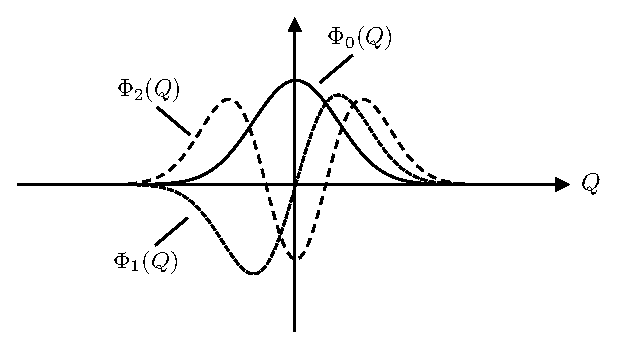
\includegraphics[width=8cm]{fig/2-2_Hermite_Gaussian.eps} 
  \caption{調和振動子のエネルギー固有状態の$Q$表示による波動関数($\Phi_0(Q), \Phi_1(Q), \Phi_2(Q)$)。}
  \label{fig:Hermite_Gaussian}
\end{figure}

\subsection{重ね合わせ状態}
前節で求めたエネルギー固有状態の波動関数は、時間とともに変化をしない解であった。ただし、シュレディンガー描像において、波動関数の位相は$\exp(-iE_kt/\hbar)$で時間とともに変化していく。

一方、式(\ref{eq:superposition_of_eigenstate})に示すように、様々な波動関数の線形結合もシュレディンガー方程式の解となる。このような複数の状態の線形結合を\textbf{重ね合わせ状態}\index{かさねあわせじょうたい@重ね合わせ状態}という。

重ね合わせ状態の例として、$\Psi(Q) = \frac 1 {\sqrt 2} (\Phi_0(Q) + \Phi_1(Q))$を考えてみよう。シュレディンガー描像では、この重ね合わせ状態は次式のように時間発展する。
\begin{equation}
  \Psi(Q, t) = \frac 1 {\sqrt 2}\left\{\Phi_0(Q)e^{-i(\omega/2) t} + \Phi_1(Q)e^{-i(3\omega/2)t}\right\} = \frac{e^{-i(\omega/2)t}}{\sqrt 2}\left\{\Phi_0(Q) + \Phi_1(Q)e^{-i\omega t}\right\}
  \label{eq:time_evolution_of_amplitude}
\end{equation}
ただし、$\Phi_0(Q)$および$\Phi_1(Q)$の固有エネルギーがそれぞれ$\hbar \omega /2$、$3\hbar \omega/2$であることを用いた。ここで、波動関数の絶対値の自乗を取り、$Q$の確率分布を求めると、次式を得る\footnote{ここでは波動関数が実数であることを用いた。波動関数の位相が位置によって異なると仮定すると、それは運動量を有していることになるので、時間とともに変化する解のはずであり、エネルギー固有状態たり得ない。したがって、エネルギー固有状態の波動関数の位相は位置によらないことから、実数で波動関数を表すことができる。}。
\begin{equation}
  \left| \Psi(Q, t)\right|^2 = \frac{1}{2}\left\{|\Phi_0(Q)|^2 + |\Phi_1(Q)|^2 + 2\Phi_0(Q)\Phi_1(Q)\cos\omega t\right\}
  \label{eq:time_evolution_of_probability}
\end{equation}
この式は以下のことを表している。図\ref{fig:Hermite_Gaussian}より、$\Phi_0(Q)$は偶関数、$\Phi_1(Q)$は奇関数であることがわかる。したがって、$\Phi_0(Q)$と$\Phi_1(Q)$を重ね合わせると、$Q>0$では強めあいの干渉、$Q < 0$では弱めあいの干渉が起こる。このため、$|\Psi(Q)|^2$は重心が$Q > 0$に偏った分布となる。この様子を図\ref{fig:superposition_state}に示す。

その後、式(\ref{eq:time_evolution_of_amplitude})で示されるように時間とともに位相が発展する。時間が$t = \pi / \omega$まで経過すると、$\Psi(Q)$は$\Phi_0(Q)$と$\Phi_1(Q)$の引き算の状態になる。このため、$|\Psi(Q)|$は重心が$Q < 0$に偏る。これを繰り返すことで、$\Psi(Q, t)$という状態は$Q$を周波数$\omega$で振動させるのである。これは、2つの波動関数のビートが生じている、と考えることができる。

次に、波動関数の位相も含めてもう少し詳しく見てみよう。時間$t = \pi/2\omega$では、式(\ref{eq:time_evolution_of_amplitude})は
\begin{equation}
  \Psi(Q) = \frac{e^{-i\pi/4}}{\sqrt 2}\left\{ \Phi_0(Q) - i \Phi_1(Q)\right\} = \frac{e^{-i\pi/4}}{\sqrt 2} \Phi_0(Q) \left\{ 1 - i\sqrt 2 Q\right\} 
\end{equation}
である。ここから$\Psi(Q)$の位相を求めると、
\begin{equation}
  \arg \Psi(Q) = -\pi/4 - \arctan \sqrt 2 Q
\end{equation}
を得る。右辺第2項から、$Q$の増加とともに位相が負に変化することがわかる。これは波数$k = \frac d {dQ} \arg \Psi(Q)$が負であることを表しており、運動量$P = \hbar k$も$-Q$の方向を向いている。同様に、時間$t = 3\pi / 2\omega$では運動量が正の値をとる。これは、図\ref{fig:classical_phase_space}(b)に示すような位相平面上の回転を表している。

ここでは$\Phi_0$と$\Phi_1$のビートで調和振動が表せることを示した。同様に考えていけば、重ね合わせの割合を変えることで振動振幅を変えることができることもわかるであろう。実際、たくさんの解を用いて重ね合わせの係数をうまく設定することで、様々な振幅の調和振動を表すことができる。これはコヒーレント状態と呼ばれるものであり、次章で説明する。

\begin{figure}
  \centering
  \includegraphics[width=8cm]{fig/2-3_superposition_state.eps} 
  \caption{重ね合わせ状態の波動関数の絶対値の自乗。$Q$の確率分布が重ね合わせの符号によって変化することがわかる。}
  \label{fig:superposition_state}
\end{figure}

\begin{comment}
$p, q$に対しては、
\begin{equation}
  \braket{\Delta \hat q^2}\braket{\Delta \hat p^2}\geq \frac{\hbar^2}{4}
\end{equation}
\begin{equation}
  \braket{\Delta \hat Q^2}\braket{\Delta \hat P^2}\geq \frac{1}{4}
\end{equation}
が成り立つ。
\end{comment}

\section{まとめ}
本章では以下の事柄について説明を行った。
\begin{itemize}
	\item シュレディンガー描像とシュレディンガー方程式。シュレディンガー描像では状態ベクトルが時間発展する。その時間発展を記述する方程式がシュレディンガー方程式である。また、時間発展に伴う状態ベクトルの変化は時間発展演算子で記述できる。
	\item ハイゼンベルグ描像とハイゼンベルグの運動方程式。ハイゼンベルグ描像では物理量の演算子を変化させることで時間発展を考える。このときの演算子の変化を記述するのがハイゼンベルグの運動方程式である。
	\item 調和振動子のハミルトニアンは位置エネルギーと運動エネルギーの和になる。
	\item 調和振動子のエネルギー固有状態は非負の整数$n$を用いて$\ket n$で表される。量子光学ではこの$n$を光子数に対応させる。
	\item 生成・消滅演算子。エネルギー固有状態をひとつづつ変化させる役割を持つ。同時に、消滅演算子は複素振幅の演算子でもある。
\end{itemize}
また、本節で説明した演算子について、表\ref{table:operator_of_quantity}にまとめた。これらは次章以降で頻繁に現れることになる。


\begin{table}
\caption{物理量の演算子とその意味}	
\begin{center}
\begin{tabular}{c c}
\hline
	演算子 & 意味 \\
	\hline \hline
	$\hat Q$ & 規格化された位置\\
	$\hat P$ & 規格化された運動量\\
	$\hat a$ & 複素振幅(エルミートではないので注意)\\
	$\hat a ^\dagger \hat a = \hat n$ & 量子数もしくは光子数\\
	$\hat a_1 = (\hat a + \hat a^\dagger)/2 = \hat Q/\sqrt 2$ & 複素振幅の実部\\
	$\hat a_2 = (\hat a - \hat a^\dagger)/2i = \hat P/\sqrt 2$ & 複素振幅の虚部\\
\hline
\end{tabular}
\label{table:operator_of_quantity}
\end{center}
\end{table}


